\section{Auswertung}
\label{sec:Auswertung}


\begin{table}
  \centering
  \caption{Maße des runden und des eckigen Stabes}
  \sisetup{table-format=3.2}
  \begin{tabular}{l
      S
      S
      }
    \toprule
    & \multicolumn{1}{c}{Runder Stab} & \multicolumn{1}{c}{Eckiger Stab} \\
    \midrule
    {$l\mathbin{/}\si{mm}$} & 592,0 &602,0\\
    {$l_{\text{Lit}}\mathbin{/}\si{mm}$} & 551,82 & 591,18\\
    {$d$\,bzw.\,$h\mathbin{/}\si{mm}$}& 10,0 & 10,0 \\
    {$m\mathbin{/}\si{g}$}& 129,4 & 167,2 \\
    {$m_{\text{Lit}}\mathbin{/}\si{g}$}&120,9 & 164,0\\
    \bottomrule
  \end{tabular}
\end{table}

Aus den bestimmten Daten der Stäbe wird die Dichte des Materials nach der Formel:
\begin{equation}
  \rho=\frac{m}{V}
\end{equation} mit $V$ = Volumen des Stabs, zu
$\rho_{\text{r}} = \qty{2783,06}{\kilo\gram\per\cubic\meter}$, sowie  $\rho_{\text{e}}=\qty{2777,41}{\kilo\gram\per\cubic\meter}$ bestimmt.
Aus dem Vergleich mit Literaturwerten \cite{Dichte} wird klar, dass es sich um Aluminium handelt.

Außerdem wird das Flächenträgheitsmoment $I_{\text{r}}$  der Stäbe bestimmt. Bei einem runden Querschnitt wird dafür die Formel \cite{flaeche}
\begin{equation}
  I_{\text{r}} = \frac{\pi (d/2)^4}{4}.
\end{equation} verwendet.
Das Flächenträgheitsmoment für den runden Stab beträgt also: 
\begin{equation*}
  I_{\text{r}} = \qty{4,91e-10}{\meter\tothe{4}}.
\end{equation*}

Das Flächenträgheitsmoment des eckigen Stabes mit quadratischem Querschnitt berechnet sich nach der Formel \cite{flaeche}:
\begin{equation}
  I_{\text{e}} = \frac{b^4}{12}.
\end{equation}
Das Flächenträgheitsmoment für den eckigen Stab beträgt also: 
\begin{equation*}
  I_{\text{e}} = \qty{8,33e-10}{\meter\tothe{4}}.
\end{equation*}.

\pagebreak

\subsection{einseitige Einspannung}
\label{subsec:einEin}
\begin{minipage}[t]{0.5\textwidth}
\begin{table}[H]
  \centering
  \caption{Messung der Biegung des\\ runden Stabs bei einseitiger Einspannung}
  \label{tab:runds}
  \sisetup{table-format=2.1}
  \begin{tabular}{S[table-format=3.0] S[table-format=1.2]}
    \toprule
    {$x \mathbin{/} \si{\milli\meter}$} & {$D(x) \mathbin{/} \si{\milli\meter}$}\\
    \midrule
    100 & 0,28\\
    125 & 0,35\\
    150 & 0,36\\
    175 & 0,45\\
    200 & 0,51\\
    225 & 0,62\\
    250 & 0,78\\
    275 & 0,93\\
    300 & 1,16\\
    325 & 1,34\\
    350 & 1,58\\
    370 & 1,78\\
    400 & 2,07\\
    425 & 2,30\\
    450 & 2,58\\
    475 & 2,79\\
    500 & 3,10\\
    525 & 3,48\\
    \bottomrule
  \end{tabular}
\end{table}
\end{minipage}
\begin{minipage}[t]{0.5\textwidth}
\begin{table}[H]
  \centering
  \caption{Messung der Biegung des\\ eckigen Stab bei einseitiger Einspannung}
  \label{tab:ecks}
  \sisetup{table-format=2.1}
  \begin{tabular}{S[table-format=3.0] S[table-format=1.2]}
    \toprule
    {$x \mathbin{/} \si{\milli\meter}$} & {$D(x) \mathbin{/} \si{\milli\meter}$}\\
    \midrule
    100 & 0,32\\
    125 & 0,46\\
    150 & 0,62\\
    175 & 0,73\\
    200 & 0,87\\
    225 & 1,03\\
    250 & 1,15\\
    275 & 1,32\\
    300 & 1,64\\
    325 & 1,86\\
    350 & 2,01\\
    375 & 2,32\\
    400 & 2,68\\
    425 & 2,90\\
    450 & 3,05\\
    475 & 3,44\\
    500 & 3,75\\
    525 & 4,11\\
    \bottomrule
  \end{tabular}
\end{table}
\end{minipage}

\bigskip

Die Masse des angehängten Gewichts beträgt beim runden Stab $m_{\text{rund}}=\qty{400}{\g}$ und beim eckigen Stab $m_{\text{eckig}}=\qty{600}{\g}$. Mit den Messwerten aus \autoref{tab:runds}
kann das Elastizitätsmodul mithilfe der Hilfsfunktion $Lx^2-\frac{x^3}{3}$ und der Formel \autoref{eqn:Biegung} berechnet werden.
Hierzu wird mit dem Pythonmodul Matplotlib \cite{matplotlib} der Y-Achsenabschnitt und die Steigung der linearen Regression $y = a*x + b$, 
sowie ihre Fehler berechnet.\\
\begin{align*}
  a_{\text{rund}} =&(0.0344 ± 0.0009) & b_{\text{rund}}=& (-0.0844 ± 0.0462)\\
  a_{\text{eckig}} =&(0.0396 ± 0,0005) & b_{\text{eckig}}=& (0.1098 ± 0.0293)\\
 \end{align*}
\begin{figure}[!htb]
  \centering
  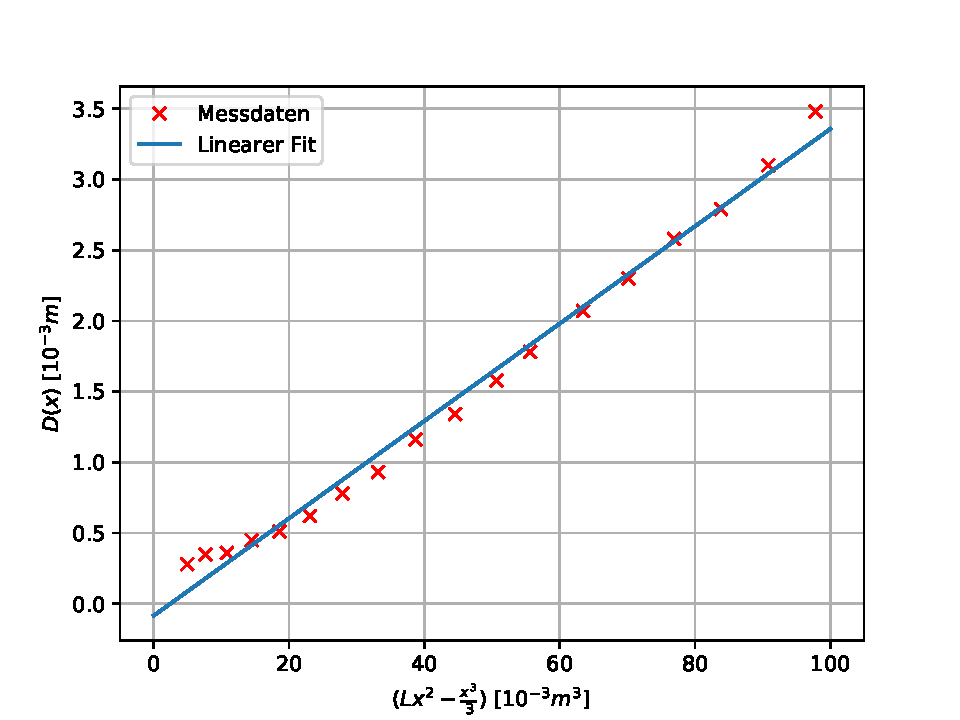
\includegraphics[scale=0.75]{content/plots/runde.pdf}
  \caption{Lineare Regression: runder Stab, einseitige Einspannung}
  \label{fig:LinRegrunde}
\end{figure}
Durch umstellen der Formel \autoref{eqn:Biegung} nach E erhält man das Elastizitätsmodul nach:
\begin{align}
    a = \frac{F}{2 \cdot E \cdot I} \iff E =\frac{m \cdot g}{2 \cdot a \cdot I}\label{eqn:Elamodul.1}
\end{align}


Nach der Gauß´schen Fehlerfortpflanzung berechnet man den Fehler durch:
\begin{equation}
  \begin{aligned}
  \Delta E &= \sqrt{\biggl(\frac{\partial E}{\partial a}\biggr)^2\cdot (\Delta a)^2} \\
  \iff \Delta E &= \frac{m\cdot g}{2\cdot I \cdot a^2} \cdot \Delta a.
  \label{eqn:e-fehler-ein}
  \end{aligned}
  \end{equation}
Somit erhält man folgende Werte für das Elastizitätsmodul:
\begin{align*}
  E_{\text{rund}}=&(11,62\pm0,03)\si{\giga\pascal}\\
  E_{\text{eckig}}=&(89,22\pm1,13)\si{\giga\pascal}\\
  \label{eqn:Eein} 
\end{align*}

\begin{figure}[!htb]
  \centering
  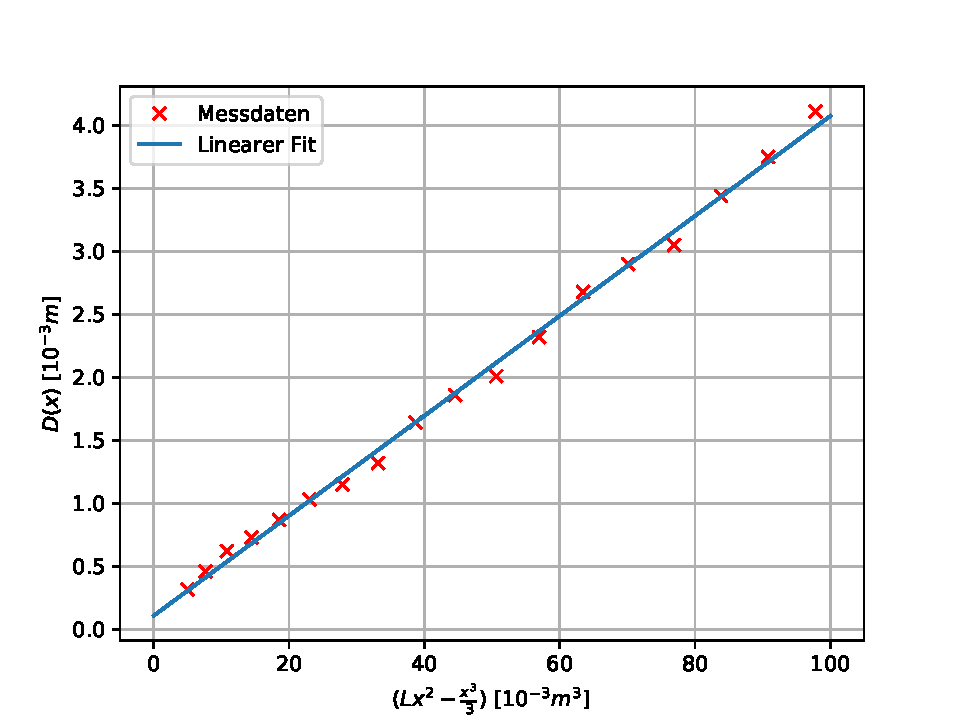
\includegraphics[scale=0.75]{content/plots/ecke.pdf}
  \caption{Lineare Regression: eckiger Stab, einseitige Einspannung}
  \label{fig:LinRegecke}
\end{figure}








\subsection{beidseitige Auflage}
\label{subsec:beidAuf}

\begin{table}[H]
  \centering
  \caption{Messung der Biegung des runden Stabs bei beidseitiger Auflage}
  \label{tab:rundb}
  \sisetup{table-format=2.1}
  \begin{tabular}{S[table-format=3.0] S[table-format=1.2]}
    \toprule
    {$x \mathbin{/} \si{\milli\meter}$} & {$D(x) \mathbin{/} \si{\milli\meter}$}\\
    \midrule
     50 & 0,15\\
     75 & 0,18\\
    100 & 0,22\\
    125 & 0,25\\
    150 & 0,31\\
    175 & 0,30\\
    200 & 0,42\\
    225 & 0,38\\
    250 & 0,40\\
    275 \\
    300 & 0,40\\
    325 & 0,37\\
    350 & 0,41\\
    375 & 0,30\\
    400 & 0,31\\
    425 & 0,25\\
    450 & 0,21\\
    475 & 0,17\\
    500 & 0,12\\
    \bottomrule
  \end{tabular}
\end{table}

\begin{figure}[H]
  \begin{subfigure}{\textwidth}
  \centering
  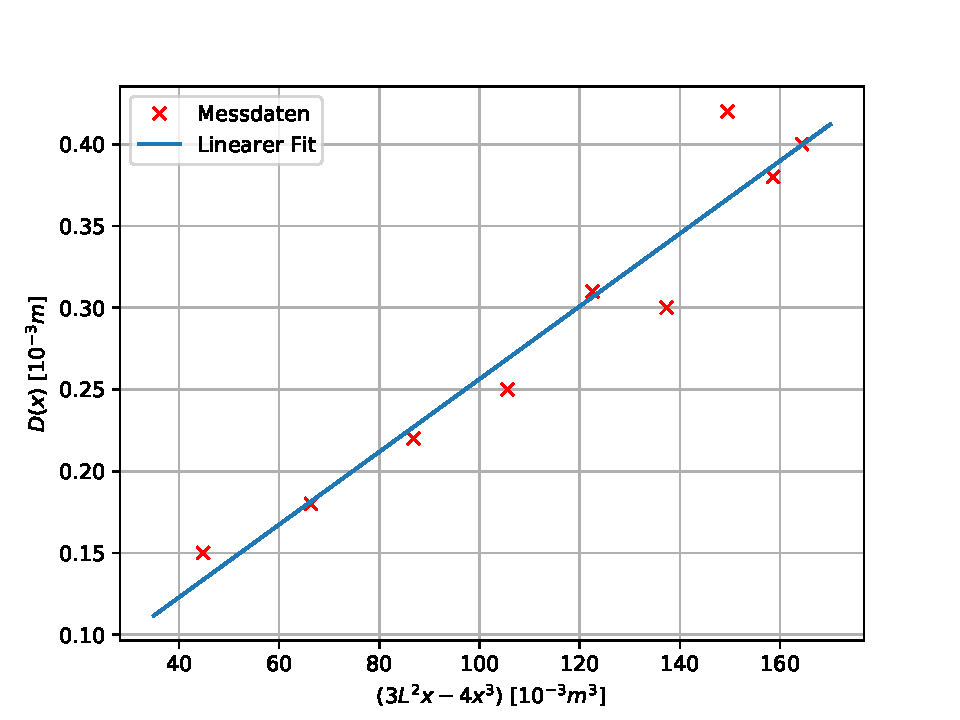
\includegraphics[height=10cm]{content/plots/rundb1.pdf}
  \caption{Lineare Regression: runder Stab, beidseitige Auflage, $0<x<L/2$}
  \label{fig:LinRegrundb1}
  \end{subfigure}
  \hfill
  \begin{subfigure}{\textwidth}
  \centering
  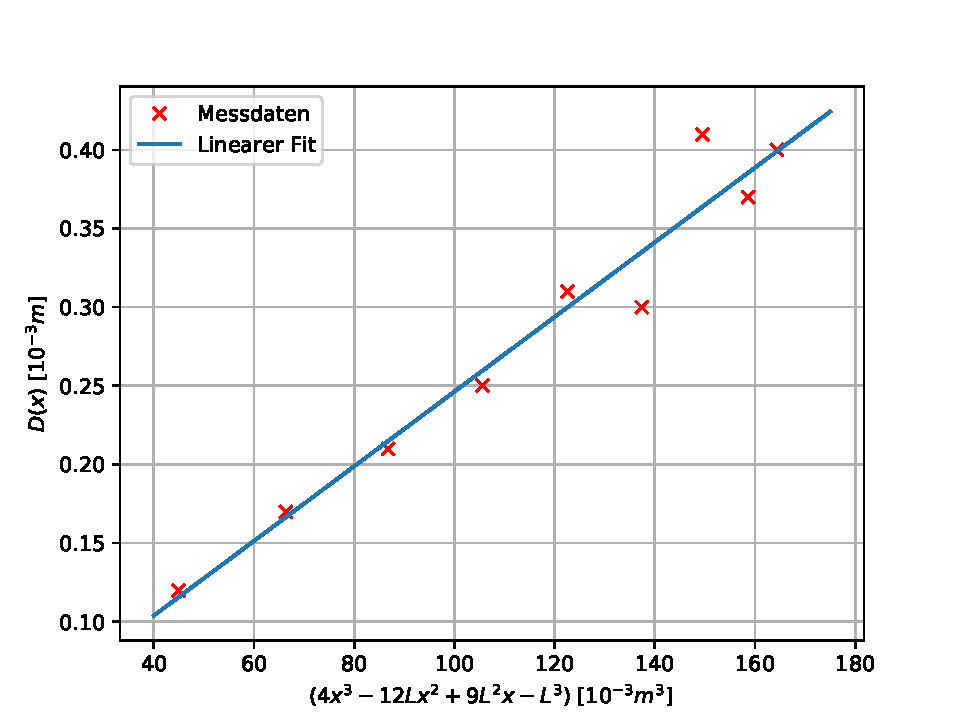
\includegraphics[height=10cm]{content/plots/rundb2.pdf}
  \caption{Lineare Regression: runder Stab, beidseitige Auflage, $x>L/2$}
  \label{fig:LinRegrundb2}
  \end{subfigure}
  \caption{Lineare Regression: runder Stab, beidseitige Auflage}
  \label{fig:LinRegrundb}
\end{figure}

\begin{table}[H]
  \centering
  \caption{Messung der Biegung des eckigen Stabs bei beidseitiger Auflage}
  \label{tab:eckb}
  \sisetup{table-format=2.1}
  \begin{tabular}{S[table-format=3.0] S[table-format=1.2]}
    \toprule
    {$x \mathbin{/} \si{\milli\meter}$} & {$D(x) \mathbin{/} \si{\milli\meter}$}\\
    \midrule
    50 & 0,01\\
    75 & 0,03\\
    100 & 0,06\\
    125 & 0,07\\
    150 & 0,08\\
    175 & 0,11\\
    200 & 0,14\\
    225 & 0,15\\
    250 & 0,16\\
    275 \\
    300 & 0,18\\
    325 & 0,17\\
    350 & 0,16\\
    375 & 0,15\\
    400 & 0,12\\
    425 & 0,12\\
    450 & 0,10\\
    475 & 0,08\\
    500 & 0,04\\
    \bottomrule
  \end{tabular}
\end{table}

\begin{figure}[H]
  \begin{subfigure}{\textwidth}
  \centering
  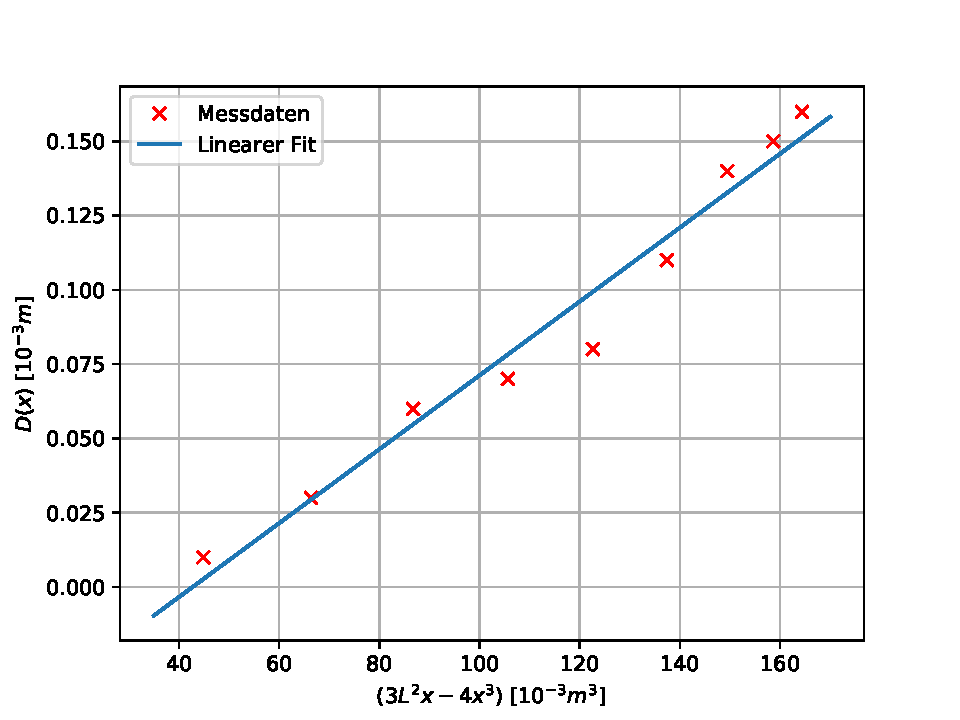
\includegraphics[height=10cm]{content/plots/eckb1.pdf}
  \caption{Lineare Regression: eckiger Stab, beidseitige Auflage, $0<x<L/2$}
  \label{fig:LinRegeckb1}
  \end{subfigure}
  \begin{subfigure}{\textwidth}
  \centering
  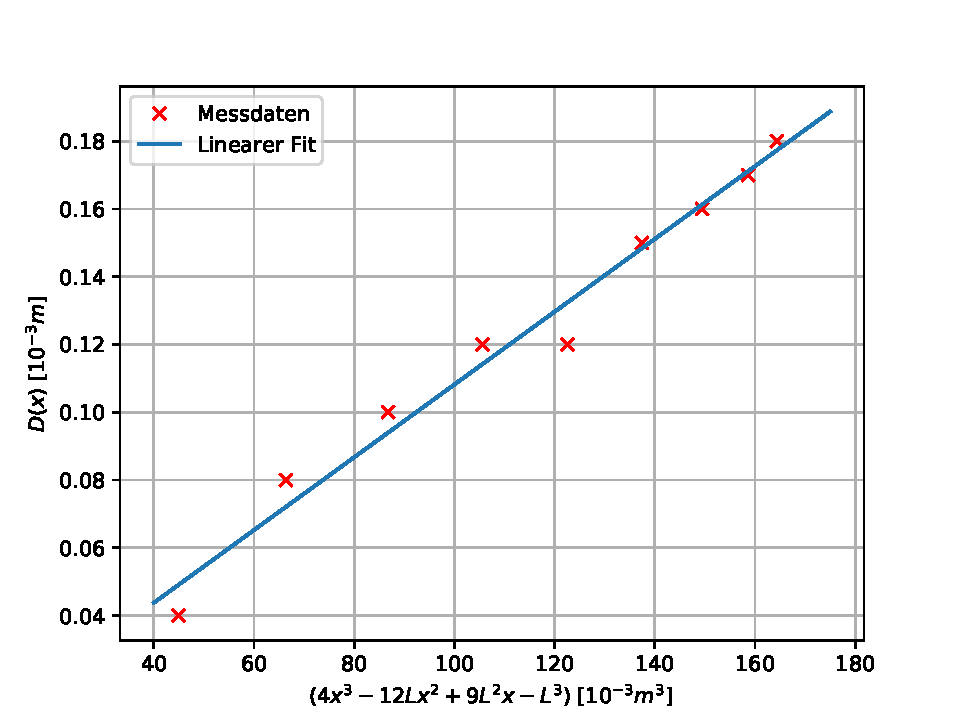
\includegraphics[height=10cm]{content/plots/eckb2.pdf}
  \caption{Lineare Regression: eckiger Stab, beidseitige Auflage, $x>L/2$}
  \label{fig:LinRegeckb2}
  \end{subfigure}
  \caption{Lineare Regression: eckiger Stab, beidseitige Auflage}
  \label{fig:LinRegeckb}
\end{figure}

Bei den beidseitig eingespannten Stäben werden dieselben Massen $m_{\text{rund}}$ und $m_{\text{eckig}}$ angehangen.
Zur Berechnung des Elastizitätsmoduls werden diesmal die Hilfsfunktion $3L^2x - 4x^3$ für den Bereich 1 $(0<x<L/2)$ und $4x^3-12Lx^2+9L^2x-L^3$ für den Bereich 2 $(x>L/2)$, sowie die Formel \autoref{eqn:Biegungb}
verwendet. Analog zu \autoref{subsec:einEin} wird auch hier Matplotlib zur Berechnung der linearen Regression genutzt.

\begin{align*}
  a_{\text{rund-1}} =&(0.0022 ± 0.0002) & b_{\text{rund-1}}=& (0.0337 ± 0.0277)\\
  a_{\text{rund-2}} =&(0.0024 ± 0.0002) & b_{\text{rund-2}}=& (0.0090 ± 0.0239)\\
  a_{\text{eckig-1}} =&(0.0012 ± 0.0001) & b_{\text{eckig-1}}=& (-0.0532 ± 0.0105)\\
  a_{\text{eckig-2}} =&(0.0011 ± 0.0001) & b_{\text{eckig-2}}=& (0.0008 ± 0.0075)\\
 \end{align*}

 Durch Umstellen der Formeln \autoref{eqn:Biegungb} nach E erhält man nun das Elastizitätsmodul:
 \begin{equation*}
  E = \frac{m\cdot g}{48\cdot I \cdot a}.
  \label{eqn:e-ein}
  \end{equation*}

Der Fehler berechnet sich nach der Gauß´schen Fehlerfortpflanzung durch:
\begin{equation*}
  \begin{aligned}
  \Delta E &= \sqrt{\biggl(\frac{\partial E}{\partial a}\biggr)^2\cdot (\Delta a)^2} \\
  \iff \Delta E &= \frac{m\cdot g}{48\cdot I \cdot a^2} \cdot \Delta a.\\
  \label{eqn:e-fehler-beid}
  \end{aligned}
  \end{equation*}

Somit beträgt das Elastizitätsmodul nun:
\begin{align*}
  E_{\text{rund-1}}=&(75,68\pm6,88)\si{\giga\pascal}\\
  E_{\text{rund-2}}=&(69,38\pm5,78)\si{\giga\pascal}\\
  E_{\text{eckig-1}}=&(122,67\pm10,22)\si{\giga\pascal}\\
  E_{\text{eckig-2}}=&(133,83\pm12,17)\si{\giga\pascal}\\
  \intertext{gemittelt zu:}
  E_{\text{rund-3}}=&(72,53\pm2,23)\si{\giga\pascal}\\
  \intertext{und}
  E_{\text{eckig-3}}=&(128,25\pm3,96)\si{\giga\pascal}\\
  \label{eqn:Ebeid} 
\end{align*}

\pagebreak



